% !TeX encoding = UTF-8
% !TeX spellcheck = en_US
\documentclass{article}
%%%%%%%%%%%%%%%%%%%%%%%%%%%%%%%%%%%%%%%%%%%%%%%%%%%%%%%%%%%%%%%%%%%%%%%%%%%%%%%%%%%%%%%%%%%%%%%%%%%%%%%%%%%%%%%%%%%%%%%%%%%%%%%%%%%%%%%%%%%%%%%%%%%%%%%%%%%%%%%%%%%%%%%%%%%%%%%%%%%%%%%%%%%%%%%%%%%%%%%%%%%%%%%%%%%%%%%%%%%%%%%%%%%%%%%%%%%%%%%%%%%%%%%%%%%%
\usepackage[
  lastexercise,
%  noanswer,
]{exercise}
\renewcommand{\QuestionNB}{\alph{Question}.\ }
\renewcommand{\subQuestionNB}{\roman{subQuestion}.\ }
\renewcommand{\subsubQuestionNB}{\arabic{subsubQuestion}.\ }

\usepackage[a4paper,top=2cm]{geometry}
\usepackage{amssymb,amsmath,amsfonts}
\usepackage[english]{babel}
\usepackage[a4paper]{geometry}
\usepackage{enumitem}
\usepackage{booktabs}
\usepackage{csquotes}
\usepackage{dcolumn}
\usepackage{graphicx}
\newcolumntype{d}[1]{D{.}{.}{#1}}

\begin{document}
	
	\title{Econometrics 1 \\ \small Exam}
	\author{Dr. Willi Mutschler}
	\date{February 16, 2018}
	\maketitle
	
	\begin{itemize}
		\item Answer \textbf{all} of the following exercises in either German or English.
		\item Explain your answers and derivations. All your computations and intermediate steps need to be verifiable and understandable. 
		\item Formulas which we covered in the lecture and class need not to be derived again.
		\item If you prefer a notation different from the one used in the course, define it.
		\item Always use significance level $a=5\%$.
		\item Please report 3 decimal places in numerical answers.
		\item If not otherwise stated, assume the validity of the assumption A, B and C given in the lecture.
		\item Permissible aids:
		\begin{itemize}
			\item non-programmable pocket calculator
			\item cheat sheet: one-sided A4 white sheet of paper with annotations, formulas, texts, sketches, etc.
		\end{itemize}
	\end{itemize}
\thispagestyle{empty}

\newpage

\setcounter{page}{1}
\begin{Exercise}[title=(Understanding)]
	\Question State one of the A, B and C assumptions introduced in the lecture in your own words. Provide a counter example by drawing a picture of points (scatterplot), if possible. Otherwise describe the counterexample in your own words.
	\Question Explain the idea of the Likelihood-Ratio test in two	sentences.	
\end{Exercise}
\begin{Answer}
	\Question
	The relationship between the endogenous variable $y_t$ and $x_t$ is linear. A counter example:
	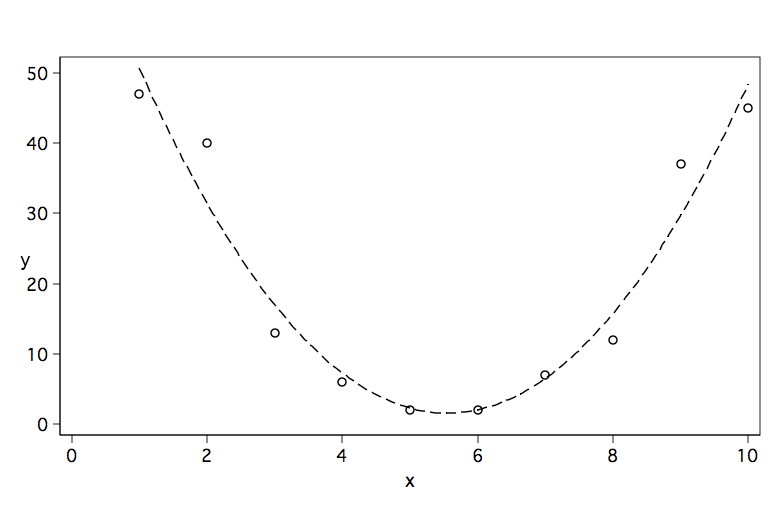
\includegraphics[width=0.5\textwidth]{plots/quadratic.png}
	
	\Question
	If the maximal likelihood under the restrictions $L(\hat{\beta}_R,\hat{\sigma}^2_R)$ is significantly lower than the maximal likelihood without restrictions $L(\hat{\beta}_{ML},\hat{\sigma}^2_{ML})$ then we reject the null hypothesis.
\end{Answer}
\newpage

\begin{Exercise}[title=(Money Demand)]
The demand for money is determined using the regression model
$$ y_t = \alpha + \beta_1 x_{1t} + \beta_2 x_{2t} + u_t$$
where
\begin{align*}
	y_t:    & \text{ real money stock in logs}\\
	x_{1t}: & \text{ real income in logs}\\
	x_{2t}: & \text{ interest rate in \%}
\end{align*} 
Given quarterly data for the period 1970-1996 ($T=108$), a least squares estimation shows that
$$\hat{y}_t = -8.2 +1.5x_{1t} - 0.01 x_{2t}$$
and $$R^2 = 0.95$$
The estimated covariance matrix of $\hat{\beta}$ is given by
$$\widehat{\operatorname{Var}}(\hat{\beta}) = \hat{\sigma}^2 (X'X)^{-1} = 
\begin{pmatrix} 
0.012 & -0.002 & 0\\
& 0.002  & 0\\
&        & 0.001			
\end{pmatrix}$$
Furthermore, we have that $$\frac{1}{T} (\mathbf{y}'\mathbf{y} - T \bar{y}^2)=20$$ where $\mathbf{y}$ denotes the $T\times1$ vector with $y_t$ in the t-th row.
\Question What do the estimated values $\hat{\beta}_1$ and $\hat{\beta}_2$ mean for the effect of the corresponding variables on the demand for money?
\Question Test the following hypotheses:
	\subQuestion $H_0:$ $\beta_1=1$ vs. $H_1: \beta_1 \neq1$
	\subQuestion $H_0:$ $\beta_2=0$ vs. $H_1: \beta_2 <0$
	\subQuestion $H_0:$ $\beta_1=1$ and $\beta_2=0$ vs. $H_1:$ the null hypothesis is not true.
\Question Compute the maximum likelihood estimators for $\alpha$, $\beta_1$, $\beta_2$ and $\sigma^2$.\\
\textit{Hint: $R^2=1-\frac{S_{\hat{u}\hat{u}}}{S_{yy}}$}.
	
\end{Exercise}

\begin{Answer}
\Question
	Both variables, real money stock and real income, are in logs, hence $\hat{\beta}_1$ is an elasticity which measure the percentage change of real money demand if the real income changes by 1\%. $\hat{\beta}_2$ measures the percentage increase of real money demand, if the interest rate increases by one point, it is a semi-elasticity.
\Question
\subQuestion $H_0: \beta_1=1$ vs. $H_1:\beta_1 \neq 1$ Two-sided test: $$t= \frac{\hat{\beta}_1 - 1}{\hat{se}(\hat{\beta}_1)} = \frac{1.5-1}{\sqrt{0.002}}=11.1$$
$t^{crit} = t_{1-\alpha/2,T-3} = 1.96$. Since $|t| > t^{crit}$, we reject the null hypothesis.
\subQuestion $H_0: \beta_2=0$ vs. $H_1:\beta_2 < 0$ One-sided test: $$t= \frac{-0.01 - 0}{\sqrt{0.001}}=-0.3165$$
$t^{crit} = t_{1-\alpha,T-3} = 1.645$. Since $t < t^{crit}$, we cannot reject the null hypothesis.
\subQuestion $H_0: \beta_1=1$ and $\beta_2=0$ vs. $H_1$: not $H_0$. F-test: $H_0:R\beta = q$ with $R=\begin{pmatrix}0 & 1 & 0\\0 & 0 & 1\end{pmatrix}$ and $q=\begin{pmatrix}1\\0\end{pmatrix}$ and $L=2$, then
$$F=\frac{(R\hat{\beta}-q)'[R(X'X)^{-1}R']^{-1}(R\hat{\beta}-q)/L}{\hat{\sigma}^2}$$
Note that we have $\hat{\sigma}^2 (X'X)^{-1}$, so 
$$F=(R\hat{\beta}-q)'[R\hat{\sigma}^2(X'X)^{-1}R']^{-1}(R\hat{\beta}-q)/L = 62.55$$
$F^{crit} = F^(1-a)_{2,101} = 3.09$. As $F>F^{crit}$ we reject the null hypothesis.
\Question $R^2 = 1-\frac{S_{\hat{u}\hat{u}}}{S_{yy}}=0.95$, $S_{\hat{u}\hat{u}} = (1-0.95)S_{yy}$, $S_{yy} = \sum (y_t -\bar{y})^2 = \sum y_t^2 - T\bar{y}^2 = 108\cdot 20 =2160$.
Hence, $S_{\hat{u}\hat{u}} = 108$, then $\hat{\sigma}^2_{ML} = \frac{1}{108}108 = 1$.

$\hat{\beta}_{1,ML} = \hat{\beta}_1 = 1.5$, $\hat{\beta}_{2,ML} = \hat{\beta}_2 = -0.01$ and $\hat{\alpha}_{ML} = \hat{\alpha} = -8.2$
\end{Answer}

\newpage

\begin{Exercise}[title=(Capital-Asset-Pricing-Model)]
Consider the following regression model for an extended Capital-Asset-Pricing-Model (CAPM):
$$y_t = \alpha + \beta_1 x_{1t} + \beta_2 x_{2t} + u_t$$
where
\begin{align*}
	y_t&: \text{rate of return of BMW in \%}\\
	x_{1t}&: \text{rate of return of the DAX index in \%}\\
	x_{2t}&: \text{price-earnings (P/E) ratio of BMW}
\end{align*}
Note that the P/E ratio is defined as the ratio of a company's stock price to the company's earnings per share. For daily observations we have the following intermediate results:
\begin{align*}
\mathbf{X}'\mathbf{X} &= 
\begin{pmatrix}
100  & 30 & 20\\
30 & 110 & 7\\
20 & 7 & 200\\
\end{pmatrix}, \\
(\mathbf{X}'\mathbf{X})^{-1} &= 
\begin{pmatrix}
0.011  & -0.003 & -0.001\\
-0.003 & 0.010 & 0\\
-0.001 & 0 & 0.005\\
\end{pmatrix},\\
\mathbf{X}'\mathbf{y}&= 
\begin{pmatrix}
29.29\\
58.79\\
45.86\\
\end{pmatrix},\\
\mathbf{y}'\mathbf{y} &= 138.496
\end{align*}

\Question Estimate a $95\%$ confidence interval for $\beta_2$ given the least squares estimator $\hat{\beta}_2$.

\Question Your professor argues that $x_{2t}$ is not a relevant variable and wants you to reestimate the model without it. Do you agree with your professor given the current dataset? Briefly outline the possible consequences of omitting $x_{2t}$.
\Question Assume that the true value of $\beta_2$ is 0.2. Compute the bias of the least squares estimators $\hat{\alpha}$ and $\hat{\beta}_1$ if one estimates
$$y_t = \alpha + \beta_1 x_{1t} + v_t$$
where $v_t$ are the error terms of the simplified regression model.\\\textit{Hint:}
$
\begin{pmatrix}
100 &  30\\
30  &110\\
\end{pmatrix}^{-1}=
\begin{pmatrix}
 0.011 &  -0.003\\
-0.003 &   0.010
\end{pmatrix}
$
\end{Exercise}

\begin{Answer}
\Question
$$\hat{\beta}=(X'X)^{-1}(X'y) = \begin{pmatrix}0.1\\0.5\\0.2\end{pmatrix}$$
$$\hat{V}(\hat{\beta}) = \hat{\sigma}^2 (X'X)^{-1}$$
Due to the variance decomposition, we have
$$\hat{u}'\hat{u} = y'y - \hat{\beta}'X'y = 138.495 - \begin{pmatrix}0.1 & 0.5 & 0.2\end{pmatrix} \begin{pmatrix} 29.29\\58.79\\45.86\end{pmatrix} = 97$$
$$\hat{\sigma}^2 = \frac{1}{100-3} \cdot 97 = 1$$
$$\hat{V}(\hat{\beta}_3) = 0.005 \hat{\sigma}^2 = 0.005$$
$$t_{1-\alpha/2} = 1.9847$$
The interval is
$$[\hat{\beta_3} \pm t_{1-\alpha/2} \hat{V}(\hat{\beta}_3)]$$
\Question
Omitted variable bias! Since $X'X$ is not diagonal, there is a bias.
\Question
We have $$E(\hat{\beta}_a)-\beta_a = (X_a'X_a)^{-1} X_a'X_2\beta_2$$
Re-estimation:
$$X'X = \begin{pmatrix} X_a'X_a & X_a'X_2\\ X_2' X_a & X_2'X_2\end{pmatrix}$$
$$(X_a'X_a)^{-1} = \begin{pmatrix} 100 & 30 \\ 30 &100 \end{pmatrix}^{-1} = \begin{pmatrix}0.011 & -0.003 \\ -0.003 & 0.010\end{pmatrix}$$
Hence the bias is equal to
$$\begin{pmatrix}0.011 & -0.003 \\ -0.003 & 0.010\end{pmatrix}\begin{pmatrix}20\\7\end{pmatrix} \cdot 0.2 = \begin{pmatrix}0.0398\\0.002\end{pmatrix}$$
\end{Answer}
\newpage

\begin{Exercise}[title=(Estimating Functions)]
Consider the simple linear regression model
$$y_t = \alpha + \beta x_t + u_t, \qquad t=1,...,20$$
and the following estimating function for the slope parameter $\beta$:
$$\tilde{\beta} = \frac{\bar{y}_2-\bar{y}_1}{\bar{x}_2 -\bar{x}_1}$$
where
$$\bar{y}_1 = \frac{1}{10} \sum_{t=1}^{10} y_t, \quad \bar{y}_2 = \frac{1}{10} \sum_{t=11}^{20} y_t, \quad \bar{x}_1 = \frac{1}{10} \sum_{t=1}^{10} x_t, \quad \bar{x}_2 = \frac{1}{10} \sum_{t=11}^{20} x_t$$
\Question Show that $\tilde{\beta}$ is an unbiased estimating function for $\beta$.\\\textit{Hint: Show that }$$\tilde{\beta} = \beta + \frac{\sum_{t=11}^{20} u_t - \sum_{t=1}^{10}u_t}{k}$$
	\textit{where $k=\sum_{t=11}^{20} x_t - \sum_{t=1}^{10} x_t$.}

\Question For the next two exercises assume that 
$$\sum_{t=1}^{20}(x_t - \bar{x})^2 = 40, \quad \sigma^2=1, \quad \bar{x}_1 = 3, \quad \bar{x}_2 = 5.$$
\subQuestion Compute the variance of $\tilde{\beta}$.\\
	\textit{Hint: Use the fact that $E(u_t u_s) = 0$ for $t\neq s$.}
\subQuestion Compute the variance of the least-squares estimator $\hat{\beta}$ and compare it to the one of $\tilde{\beta}$.
\end{Exercise}

\begin{Answer}
\Question
We need to show that $E(\tilde{\beta}) = \beta$. Proof:
\begin{align*}
\tilde{\beta} &= \frac{\bar{y}_2 - \bar{y}_1}{\bar{x}_2 - \bar{x}_1}\\
&= \frac{1/10 \sum_{t=11}^{20} y_t - 1/10 \sum_{t=1}^{10} y_t}{1/10 \sum_{t=11}^{20} x_t - 1/10 \sum_{t=1}^{10} x_t}\\
&= \frac{\sum_{t=11}^{20} y_t - \sum_{t=1}^{10} y_t}{\sum_{t=11}^{20} x_t - \sum_{t=1}^{10} x_t}\\
&= \frac{\sum_{t=11}^{20} (\alpha + \beta x_t + u_t) - \sum_{t=1}^{10} (\alpha + \beta x_t + u_t)}{\sum_{t=11}^{20} x_t - \sum_{t=1}^{10} x_t}\\
&= \frac{10\alpha + \beta \sum_{t=11}^{20} x_t + \sum_{t=11}^{20} u_t - 10 \alpha -\beta \sum_{t=1}^{10} x_t -\sum_{t=1}^{10} u_t}{\sum_{t=11}^{20} x_t - \sum_{t=1}^{10} x_t}\\
&= \frac{\beta (\sum_{t=11}^{20} x_t -\sum_{t=1}^{10} x_t) + \sum_{t=11}^{20} u_t  -\sum_{t=1}^{10} u_t}{\sum_{t=11}^{20} x_t - \sum_{t=1}^{10} x_t}\\
&= \beta + \frac{\sum_{t=11}^{20} u_t  -\sum_{t=1}^{10} u_t}{\sum_{t=11}^{20} x_t - \sum_{t=1}^{10} x_t}
\end{align*}
Since $E(u_t)=0$, we have that 
$$E(\tilde{\beta}) = \beta$$
\Question
\subQuestion
\begin{align*}
var(\tilde{\beta}) &= E[(\tilde{\beta}-E(\tilde{\beta}))^2] = E[(\tilde{\beta}-\beta)^2] = E\left[\left( \frac{\sum_{t=11}^{20} u_t  -\sum_{t=1}^{10} u_t}{\sum_{t=11}^{20} x_t - \sum_{t=1}^{10} x_t}\right)\right]\\
&=\frac{1}{(\sum_{t=11}^{20} x_t - \sum_{t=1}^{10} x_t)^2}\cdot E\left[\sum_{t=11}^{20}u_t\sum_{t=11}^{20}u_t - 2\sum_{t=11}^{20}u_t\sum_{t=1}^{10}u_t + \sum_{t=1}^{10}u_t\sum_{t=1}^{10}u_t\right]
\end{align*}
Note that $E[u_tu_s]=$ for $t\neq s$, hence
\begin{align*}
\tilde{\beta} &= \frac{1}{(\sum_{t=11}^{20} x_t - \sum_{t=1}^{10} x_t)^2}\cdot \left[\sum_{t=11}^{20}E[u_t^2] + \sum_{t=1}^{10}E[u_t^2]\right]\\
&= \frac{1}{(\sum_{t=11}^{20} x_t - \sum_{t=1}^{10} x_t)^2}\cdot \left[10\sigma^2+10\sigma^2\right] = \frac{20\sigma^2}{(\sum_{t=11}^{20} x_t - \sum_{t=1}^{10} x_t)^2}
\end{align*}
We have that $\bar{x}_1 \cdot 10 = \sum_{t=1}^{10} x_t = 3\cdot 10 = 30$ and $\sum_{t=11}^{20} x_t = 5 \cdot 10 = 50$. Hence
$$var(\tilde{\beta}) = \frac{20 \cdot 1}{(50-30)^2} = \frac{1}{20}$$
\subQuestion
Variance of OLS estimator: $$var(\hat{\beta}) = \frac{\sigma^2}{\sum_{t=1}^{20}(x_t-\bar{x})^2} = \frac{1}{40}$$
OLS is BLUE, hence it has a smaller variance that $\tilde{\beta}$.
\end{Answer}

\newpage 
	\begin{minipage}[t]{6cm}
		Table of quantiles of the $t_{\nu }$-distribution,\\ given are the $(1-a)$%
		-quantiles
		
		\begin{center}
			\begin{tabular}{|r|rrr|}
				\hline
				& \multicolumn{3}{|c|}{$a$} \\ 
				$\nu$ & 0.05 & 0.025 & 0.01 \\ \hline
				1 & 6.31380 & 12.70620 & 31.82050 \\
				2 & 2.92000 & 4.30270 & 6.96460 \\
				3 & 2.35340 & 3.18240 & 4.54070 \\
				4 & 2.13180 & 2.77640 & 3.74690 \\
				5 & 2.01500 & 2.57060 & 3.36490 \\
				6 & 1.94320 & 2.44690 & 3.14270 \\
				7 & 1.89460 & 2.36460 & 2.99800 \\
				8 & 1.85950 & 2.30600 & 2.89650 \\
				9 & 1.83310 & 2.26220 & 2.82140 \\
				10 & 1.81250 & 2.22810 & 2.76380 \\
				11 & 1.79590 & 2.20100 & 2.71810 \\
				12 & 1.78230 & 2.17880 & 2.68100 \\
				13 & 1.77090 & 2.16040 & 2.65030 \\
				14 & 1.76130 & 2.14480 & 2.62450 \\
				15 & 1.75310 & 2.13140 & 2.60250 \\
				16 & 1.74590 & 2.11990 & 2.58350 \\
				17 & 1.73960 & 2.10980 & 2.56690 \\
				18 & 1.73410 & 2.10090 & 2.55240 \\
				19 & 1.72910 & 2.09300 & 2.53950 \\
				20 & 1.72470 & 2.08600 & 2.52800 \\
				21 & 1.72070 & 2.07960 & 2.51760 \\
				22 & 1.71710 & 2.07390 & 2.50830 \\
				23 & 1.71390 & 2.06870 & 2.49990 \\
				24 & 1.71090 & 2.06390 & 2.49220 \\
				25 & 1.70810 & 2.05950 & 2.48510 \\
				26 & 1.70560 & 2.05550 & 2.47860 \\
				27 & 1.70330 & 2.05180 & 2.47270 \\
				28 & 1.70110 & 2.04840 & 2.46710 \\
				29 & 1.69910 & 2.04520 & 2.46200 \\
				30 & 1.69730 & 2.04230 & 2.45730 \\
				31 & 1.69550 & 2.03950 & 2.45280 \\
				32 & 1.69390 & 2.03690 & 2.44870 \\
				33 & 1.69240 & 2.03450 & 2.44480 \\
				34 & 1.69090 & 2.03220 & 2.44110 \\
				35 & 1.68960 & 2.03010 & 2.43770 \\
				36 & 1.68830 & 2.02810 & 2.43450 \\
				37 & 1.68710 & 2.02620 & 2.43140 \\
				38 & 1.68600 & 2.02440 & 2.42860 \\
				39 & 1.68490 & 2.02270 & 2.42580 \\
				40 & 1.68390 & 2.02110 & 2.42330 \\
				$>40$& 1.645 & 1.960 & 2.326 \\ \hline
			\end{tabular}
		\end{center}
	\end{minipage}\hspace{2cm} 
	\begin{minipage}[t]{6cm}
		Table of quantiles of the $\chi^2_{\nu }$-distribution, given are $(1-a)$-quantiles
		
		\begin{center}
			\begin{tabular}{|r|rrr|}
				\hline
				& \multicolumn{3}{|c|}{$a$} \\ 
				$\nu$ & 0.05 & 0.025 & 0.01 \\ \hline
				1 & 3.84 & 5.02 & 6.63 \\
				2 & 5.99 & 7.38 & 9.21 \\
				3 & 7.82 & 9.35 & 11.35 \\
				4 & 9.49 & 11.14 & 13.28 \\
				5 & 11.07 & 12.83 & 15.09 \\
				6 & 12.59 & 14.45 & 16.81 \\
				7 & 14.07 & 16.01 & 18.48 \\
				8 & 15.51 & 17.54 & 20.09 \\
				9 & 16.92 & 19.02 & 21.67 \\
				10 & 18.31 & 20.48 & 23.21 \\
				11 & 19.68 & 21.92 & 24.73 \\
				12 & 21.03 & 23.34 & 26.22 \\
				13 & 22.36 & 24.74 & 27.69 \\
				14 & 23.68 & 26.12 & 29.14 \\
				15 & 25.00 & 27.49 & 30.58 \\
				16 & 26.30 & 28.84 & 32.00 \\
				17 & 27.59 & 30.19 & 33.41 \\
				18 & 28.87 & 31.53 & 34.81 \\
				19 & 30.14 & 32.85 & 36.19 \\
				20 & 31.41 & 34.17 & 37.57 \\
				21 & 32.67 & 35.48 & 38.93 \\
				22 & 33.92 & 36.78 & 40.29 \\
				23 & 35.17 & 38.08 & 41.64 \\
				24 & 36.41 & 39.36 & 42.98 \\
				25 & 37.65 & 40.65 & 44.31 \\
				26 & 38.88 & 41.92 & 45.64 \\
				27 & 40.11 & 43.20 & 46.96 \\
				28 & 41.34 & 44.46 & 48.28 \\
				29 & 42.56 & 45.72 & 49.59 \\
				30 & 43.77 & 46.98 & 50.89 \\
				35 & 49.80 & 53.20 & 57.34 \\
				40 & 55.76 & 59.34 & 63.69 \\
				45 & 61.66 & 65.41 & 69.96 \\
				50 & 67.50 & 71.42 & 76.15 \\
				55 & 73.31 & 77.38 & 82.29 \\
				60 & 79.08 & 83.30 & 88.38 \\
				65 & 84.82 & 89.18 & 94.42 \\
				70 & 90.53 & 95.02 & 100.43 \\
				75 & 96.22 & 100.84 & 106.39 \\
				80 & 101.88 & 106.63 & 112.33 \\
				85 & 107.52 & 112.39 & 118.24 \\
				90 & 113.15 & 118.14 & 124.12 \\
				95 & 118.75 & 123.86 & 129.97 \\
				100 & 124.34 & 129.56 & 135.81 \\ \hline
			\end{tabular}
		\end{center}
	\end{minipage}\newpage Table of the quantiles of the $F_{\nu _{1},\nu _{2}}$%
	-distribution,	given are the 0.95 -quantiles (i.e. $a=0.05$)
	
	\begin{tabular}{|r|rrrrrrrrrr|}
		\hline
		& \multicolumn{10}{|c|}{$\nu_1$} \\ 
		$\nu_2$ & 1 & 2 & 3 & 4 & 5 & 10 & 15 & 20 & 25 & 50 \\ \hline
		1 & 161.45 & 199.50 & 215.71 & 224.58 & 230.16 & 241.88 & 245.95 & 248.01 & 
		249.26 & 251.77 \\ 
		2 & 18.51 & 19.00 & 19.16 & 19.25 & 19.30 & 19.40 & 19.43 & 19.45 & 19.46 & 
		19.48 \\ 
		3 & 10.13 & 9.55 & 9.28 & 9.12 & 9.01 & 8.79 & 8.70 & 8.66 & 8.63 & 8.58 \\ 
		4 & 7.71 & 6.94 & 6.59 & 6.39 & 6.26 & 5.96 & 5.86 & 5.80 & 5.77 & 5.70 \\ 
		5 & 6.61 & 5.79 & 5.41 & 5.19 & 5.05 & 4.74 & 4.62 & 4.56 & 4.52 & 4.44 \\ 
		6 & 5.99 & 5.14 & 4.76 & 4.53 & 4.39 & 4.06 & 3.94 & 3.87 & 3.83 & 3.75 \\ 
		7 & 5.59 & 4.74 & 4.35 & 4.12 & 3.97 & 3.64 & 3.51 & 3.44 & 3.40 & 3.32 \\ 
		8 & 5.32 & 4.46 & 4.07 & 3.84 & 3.69 & 3.35 & 3.22 & 3.15 & 3.11 & 3.02 \\ 
		9 & 5.12 & 4.26 & 3.86 & 3.63 & 3.48 & 3.14 & 3.01 & 2.94 & 2.89 & 2.80 \\ 
		10 & 4.96 & 4.10 & 3.71 & 3.48 & 3.33 & 2.98 & 2.85 & 2.77 & 2.73 & 2.64 \\ 
		15 & 4.54 & 3.68 & 3.29 & 3.06 & 2.90 & 2.54 & 2.40 & 2.33 & 2.28 & 2.18 \\ 
		20 & 4.35 & 3.49 & 3.10 & 2.87 & 2.71 & 2.35 & 2.20 & 2.12 & 2.07 & 1.97 \\ 
		25 & 4.24 & 3.39 & 2.99 & 2.76 & 2.60 & 2.24 & 2.09 & 2.01 & 1.96 & 1.84 \\ 
		30 & 4.17 & 3.32 & 2.92 & 2.69 & 2.53 & 2.16 & 2.01 & 1.93 & 1.88 & 1.76 \\ 
		35 & 4.12 & 3.27 & 2.87 & 2.64 & 2.49 & 2.11 & 1.96 & 1.88 & 1.82 & 1.70 \\ 
		40 & 4.08 & 3.23 & 2.84 & 2.61 & 2.45 & 2.08 & 1.92 & 1.84 & 1.78 & 1.66 \\ 
		45 & 4.06 & 3.20 & 2.81 & 2.58 & 2.42 & 2.05 & 1.89 & 1.81 & 1.75 & 1.63 \\ 
		50 & 4.03 & 3.18 & 2.79 & 2.56 & 2.40 & 2.03 & 1.87 & 1.78 & 1.73 & 1.60 \\ 
		55 & 4.02 & 3.16 & 2.77 & 2.54 & 2.38 & 2.01 & 1.85 & 1.76 & 1.71 & 1.58 \\ 
		60 & 4.00 & 3.15 & 2.76 & 2.53 & 2.37 & 1.99 & 1.84 & 1.75 & 1.69 & 1.56 \\ 
		65 & 3.99 & 3.14 & 2.75 & 2.51 & 2.36 & 1.98 & 1.82 & 1.73 & 1.68 & 1.54 \\ 
		70 & 3.98 & 3.13 & 2.74 & 2.50 & 2.35 & 1.97 & 1.81 & 1.72 & 1.66 & 1.53 \\ 
		75 & 3.97 & 3.12 & 2.73 & 2.49 & 2.34 & 1.96 & 1.80 & 1.71 & 1.65 & 1.52 \\ 
		80 & 3.96 & 3.11 & 2.72 & 2.49 & 2.33 & 1.95 & 1.79 & 1.70 & 1.64 & 1.51 \\ 
		85 & 3.95 & 3.10 & 2.71 & 2.48 & 2.32 & 1.94 & 1.79 & 1.70 & 1.64 & 1.50 \\ 
		90 & 3.95 & 3.10 & 2.71 & 2.47 & 2.32 & 1.94 & 1.78 & 1.69 & 1.63 & 1.49 \\ 
		95 & 3.94 & 3.09 & 2.70 & 2.47 & 2.31 & 1.93 & 1.77 & 1.68 & 1.62 & 1.48 \\ 
		100 & 3.94 & 3.09 & 2.70 & 2.46 & 2.31 & 1.93 & 1.77 & 1.68 & 1.62 & 1.48 \\ 
		\hline
	\end{tabular}
	
\end{document}
